\subsection{Iterator}
\subsubsection{Định nghĩa}
Iterator là một mẫu thiết kế hành vi (behavioral design pattern) cho phép truy cập tuần tự vào các phần tử của một tập hợp (collection) mà không tiết lộ cấu trúc nội bộ của nó. Nó cung cấp một cách tiếp cận thống nhất để duyệt qua các phần tử của một tập hợp mà không phụ thuộc vào kiểu cấu trúc dữ liệu của tập hợp đó.
\subsubsection{Cách sử dụng}
Ta sẽ sử dụng Pattern này trong các trường hợp:
\begin{itemize}
    \item Sử dụng mẫu Iterator khi collection của bạn có một cấu trúc dữ phức tạp, nhưng bạn muốn ẩn tính phức tạp chung của nó với các máy khác (để thuận tiện hoặc bảo mật).
    \item Khi được đặt trong logic kinh doanh của một ứng dụng, nó có thể làm lu mờ vai trò của source code gốc và làm cho nó khó bảo trì hơn. Với việc di chuyển source code đó đến các Iterator được chỉ định có thể giúp code của mình gọn gàng và sạch sẽ hơn.
    \item Sử dụng Iterator khi bạn muốn có một interface duy nhất để duyệt qua các phần tử của một tập hợp, code của mình có thể follow các cấu trúc dữ liệu khác nhau hoặc khi các loại cấu trúc chuỗi này chưa được biết trước.
\end{itemize}
\subsubsection{Cấu trúc}
\begin{center}
    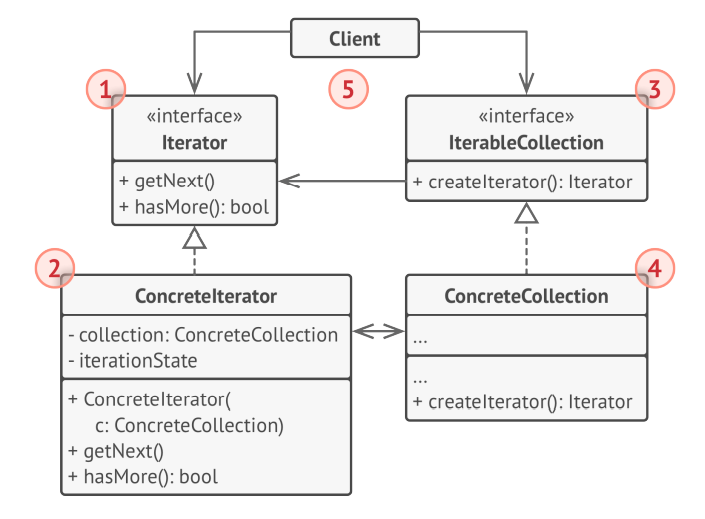
\includegraphics[scale= 0.6]{image/behavioral/iterator.png}
\end{center}
Các thành phần chính:
\begin{itemize}
    \item Một interface hay abstract class tên Iterator định nghĩa các hoạt động cần thiết.
    \item Concrete Iterator implement các phương thức trên.
    \item Collection Interface để khai báo một hoặc nhiều phương thức để nhận được các Iterator tương thích với collection.
    \item Concrete Collection trả về các phiên bản của một lớp Iterator cụ thể mỗi khi có các dòng code yêu cầu.
\end{itemize}
\subsubsection{Ưu điểm và Nhược điểm}
Có các ưu điểm và nhược điểm sau:
Ưu điểm:
\begin{itemize}
    \item Hỗ trợ nhiều cách duyệt qua các phần tử, bao gồm duyệt theo chiều thuận, chiều ngược và duyệt ngẫu nhiên.
    \item Chúng ta có thể truy cập song song trên cùng một tập hợp vì mỗi đối tượng iterator có chứa trạng thái riêng của nó.
\end{itemize}
Nhược điểm:
\begin{itemize}
    \item Sử dụng iterator có thể kém hiệu quả hơn so với việc duyệt qua các phần tử của bộ sưu tập một cách trực tiếp.
    \item Có thể không cần thiết nếu ứng dụng chỉ hoạt động với các collection đơn giản.
\end{itemize}
\subsubsection{Code Example}
\begin{itemize}
    \item Một interface Iterator và một VectorIterator là subclass.
\end{itemize}
\begin{lstlisting}
#include <iostream>
#include <vector>

// Iterator interface
class Iterator {
public:
    virtual bool hasNext() = 0;
    virtual int next() = 0;
};

// Concrete iterator
class VectorIterator : public Iterator {
private:
    std::vector<int>& vector;
    int index;

public:
    VectorIterator(std::vector<int>& vec) : vector(vec), index(0) {}

    bool hasNext() override {
        return index < vector.size();
    }

    int next() override {
        return vector[index++];
    }
};

// Client code
void printValues(Iterator& iterator) {
    while (iterator.hasNext()) {
        std::cout << iterator.next() << " ";
    }
    std::cout << std::endl;
}

int main() {
    std::vector<int> numbers = { 1, 2, 3, 4, 5 };
    VectorIterator iterator(numbers);

    printValues(iterator);

    return 0;
}

\end{lstlisting}
Ở hàm main, ta gọi một vector int là dùng iterator duyệt qua các giá trị đó.\\
\newline
\textbf{Kết quả:}
\begin{lstlisting}
1 2 3 4 5 
\end{lstlisting}
\subsubsection{Các Pattern liên quan}
\begin{itemize}
    \item Composite: ta thường dùng Iterator để duyệt qua cấu trúc cây.
    \item Memento: có thể kết hợp với Memento để lưu lại các trạng thái đã từng duyệt qua.
    \item Visitor: có thể kết hợp với Iterator để xem qua một cấu trúc dữ liệu phức tạp và thực hiện một số thao tác trên các phần tử của nó.
\end{itemize}
